\documentclass[letterpaper,12pt]{exam}

\RequirePackage{comment}
\RequirePackage[hypertex]{hyperref}
\RequirePackage{GE05}
% this inputs graphicx, too
\usepackage{booktabs}

\newcommand{\NX}{\mbox{\em NX\/}}
\newcommand{\POP}{\mbox{\em POP\/}}

\def\ClassName{The Global Economy}
\def\Category{Professor David Backus}
\def\HeadName{Final Examination}

\printanswers 

\begin{document}
\parindent = 0.0in
\parskip = \bigskipamount
\thispagestyle{empty}%
\Head

\centerline{\large \bf \HeadName}%
%\centerline{March 9, 2005}
\centerline{Revised:  \today}

\bigskip
You have 120 minutes to complete this exam.  Please answer each
question in the space provided. You may consult one page of notes
and a calculator, but devices capable of wireless transmission are
prohibited.

I understand that the honor code applies: I will not lie, cheat,
or steal to gain an academic advantage, or tolerate those who do.

\begin{flushright}
\rule{4in}{0.5pt} \\ (Name and Signature)
\end{flushright}

%\begin{figure}[h]
%    \centering
%    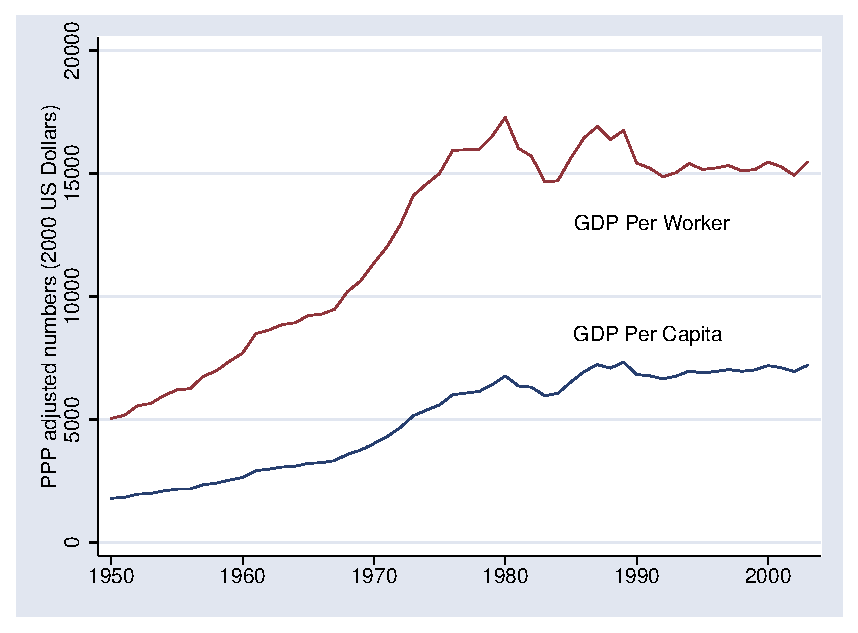
\includegraphics[scale=0.8]{pwtbramidterm07.eps}
%    \caption{GDP Per Capita and GDP Per Worker in Brazil.}
%    \label{fig:brazil}
%\end{figure}

\begin{questions}
% ======================================================================
\question {\it US monetary policy (30 points).\/} 
%
The Federal Reserve's Federal Open Market Committee (FOMC)
met April 27-28, 2010, and released this statement:  
% 
\begin{quote}
Information received since the FOMC met in March suggests that economic activity has continued to strengthen and that the labor market is beginning to improve. Growth in household spending has picked up recently.  ... 
Business spending on equipment and software has risen significantly. ...
Housing starts have edged up but remain at a depressed level. ...  
%Although the pace of economic recovery is likely to be moderate for a time, 
With substantial resource slack ... and longer-term inflation expectations stable, inflation is likely to be subdued for some time. ...

The Committee will maintain the target range for the federal funds rate at 0 to 1/4 percent.  ...

Voting against the policy action was [Kansas City Fed President] 
Thomas M. Hoenig, who believed that ... [an] exceptionally low level 
of the federal funds rate ...  was no longer warranted.  
\end{quote}
%
Later the same week, the Bureau of Economic Analysis announced that 
in the first quarter real GDP growth was estimated to be 3.2\% and 
inflation (in the GDP price index) 0.9\%.
Both are expressed at annual rates.

\begin{parts}
\part Consider this information in the context of 
the aggregate supply and demand framework.  
Based on the FOMC statement, 
where is the short-run equilibrium of the economy relative to 
the Fed's inflation target and the long-run equilibrium level of output? 
Illustrate your answer with the appropriate diagram.  
(10~points)

\part Given your answer to (a), what should the Fed's response be?  
How should it change the money supply?  The fed funds rate?  
(10~points) 

\part What would the Taylor Rule suggest for current monetary policy?  
Is it consistent with your answer to (b)?  
Given your answer(s), do you agree with Hoenig?
Why or why not?  
(10~points) 
\end{parts}   

\begin{solution}
\begin{parts} 
\part The phrase ``substantial resource slack'' 
suggests that output is below its long-run equilibrium.  
The phrase ``inflation is likely to be subdued for some time''
suggests that inflation is below target (2\% say).  
That suggests a picture something like this, with A as the short-run equilibrium and C as the target.  
%
%%%%%%%%%%%%%%%%%%%%%%%%%%%%%%%%%%%%%%%%%%%%%%%%%%%%%%%%%%%%%%%%%%%%%%%%%%%%
%  Supply and demand diagram 
%\begin{figure}[h!]
%
\begin{center}
\setlength{\unitlength}{0.075em}
\begin{picture}(300,220)(0,-20)
%\footnotesize
\thicklines

% horizontal axis
\put(-30,0){\vector(1,0){300}}
\put(255,-16){$Y$}
\put(142,-16){$Y^*$}

% vertical axis
\put(0,-20){\vector(0,1){200}}
\put(-15,155){$P$}

% demand
\put(25,165){\line(4,-3){200}}\put(230,10){AD}

% supply
\put(25,13){\line(4,3){200}} \put(230,160){AS}
\put(146.4,0){\line(0,1){170}} \put(138,175){AS$^*$}

% equilibrium labels
\put(105,85){\footnotesize A}
\put(135,60){\footnotesize B}
\put(135,110){\footnotesize C}
% dotted lines 
%\qbezier[31]{(133,0)(133,46)(133,92)}
%\qbezier[45]{(0,92)(67,92)(133,92)}
%\qbezier[45]{(0,72)(67,72)(133,72)}

\end{picture}
\end{center}
%%%%%%%%%%%%%%%%%%%%%%%%%%%%%%%%%%%%%%%%%%%%%%%%%%%%%%%%%%%%%%%%%%%%%%%%%%%%
%\bigskip 
(We don't know that C is at the intersection of AS and AS$^*$, 
just that it's above and to the right of A.) 

Grading:  10 points for something like this.  

\part The goals of policy are (i)~stable prices 
(ie, 2\% inflation) and 
(ii)~long-run equilibrium level of output. 
From (a), we know that both are below their target levels.  
We can move both in the right direction by shifting the AD curve up and
to the right.  
An increase in the money supply has this effect.
Typically we would describe this as a drop in the short-term 
``fed funds'' rate.  

Grading:  5 points for the goals, 5 for showing how the Fed would 
accomplish them.  

\part Now we shift gears and think in terms of the Taylor Rule.
The rule gives us a fed funds rate of 
\begin{eqnarray*}
    i &=& r + \pi + 0.5 (\pi - \pi^*) + 0.5 (g - g^*) \\
        &=&  2 + 0.9 + 0.5 (0.9 - 2) + 0.5 (3.2 - 3) 
        \;\;=\;\; 2.45.  
\end{eqnarray*}
There are lots of choices here, but they should give you 
an interest rate above the current recommendation of 
``0 to 1/4 percent.''

Here are some possible interpretations:  
\begin{itemize}
\item The current rate is too low.  Hoenig hints at this in his statement.
(In fact, he was making a more subtle point about whether the Fed should
commit to a long period of very low interest rates, but I edited that out
to keep things simple.) 

\item There's a difference between excess capacity ($y-y^*$) and the growth rate version we've used.  
    This is a subtle issue, not something I'd expect you to worry about, 
    but might show up in public discussion.  
    The difficulty with the capacity version is coming up with a number
    for $y^*$.  
    If you do this, you might argue that although 
    growth is now up to its postwar average,
    output remains well below its long-run equilibrium.
    That's in fact what the statement says, so this is a plausible
    interpretation of the policy decision. 
\end{itemize} 

Grading:  5 points for correct calculation of interest rate implied by 
 Taylor Rule, 5 points for a sensible discussion of what this means 
 to the Fed right now.  

\end{parts} 
\end{solution} 


%\pagebreak \phantom{xx} \pagebreak %\phantom{xx} \pagebreak
% ======================================================================
\question {\it Near-term prospects for Turkey (40 points).\/}

\begin{center}
\begin{tabular}{lrrrrrrr}
\toprule 
         &  2004  &  2005  &  2006   & 2007  & 2008 &  2009  &  2010 \\%
\midrule 
Real GDP growth  & 9.6 & 8.4 & 6.9 & 4.7 & 0.7 & --4.7 & 4.0 \\
Inflation   & 8.6 & 8.2 & 9.6 & 8.8 & 10.4 & 6.3 & 10.0 \\
TFP growth  & 6.1 & 4.7 & 4.3 & 5.7 & --2.4 & --5.7 & 2.2 \\ 
Investment rate & 20.2 & 21.0 & 22.3 & 21.4 & 19.9 & 16.8 & 15.9 \\
Saving rate     & 19.4 & 20.0 & 22.0 & 21.1 & 21.8 & 14.8 & 16.0 \\
Current account & --3.7 & --4.6 & --6.0 & --5.8 & --5.6 & --2.3 & --4.0 \\
%Trade balance   &             
Budget balance  & --5.4 & --1.3 & --0.6 & --1.6 & --1.8 & --5.5 & --5.3 \\ 
Primary balance & 4.7 & 5.8 & 5.5 & 4.2 & 3.5 & 0.1 & --0.1 \\
Public debt      & 56.6 & 51.1 & 45.5 & 39.6 & 40.0 & 46.3 \\
Net foreign assets   & --41 & --35 & --39 & --39 & --38 & --44 & --40 \\%
Interest rate:  short & 21.4 & 14.7 & 15.6 & 17.2 & 16.0 & 9.2 & 10.0\\
%Interest rate:  long  &  \\
Real exchange rate & 131 & 146 & 145 & 159 & 162 & 150 & 165 \\
Reserves           &  37 & 52 & 63 & 77 & 74 & 75 \\
\bottomrule 
\end{tabular}
\end{center}
{\it 
Economic indicators for Turkey.  
(i)~Investment, saving, current account, budget balances, 
public debt, and net foreign assets are expressed as 
percentages of GDP (ratio to GDP multiplied by 100).  
(ii)~Government budget numbers (budget balance, primary balance): 
negative numbers indicate deficits, 
positive numbers indicate surpluses.  
(iii)~The real exchange rate is a weighted average across trading partners, 
with weights tied to the amount of trade;
high numbers indicate that prices of local goods are high relative to 
prices in other countries.
(iv)~Foreign exchange reserves are expressed in billions of USD.  
(v)~2010 numbers are estimates.
All numbers courtesy of the Economist Intelligence Unit.} 

You have been asked to write a short report summarizing 
economic prospects in Turkey over the next 2-3 years.  
Is Turkey more likely to grow like China or collapse like Greece?  
Its level of development is between the two, 
with GDP per capita double China but less than half of Greece. 

Having some experience with such situations, 
you study the Economist Intelligence Unit's 
various reports and summarize the relevant sections:  
%
\begin{itemize}
\item Modern Turkish politics has evolved from the secular 
single-party republic established by Mustafa Kemal (Ataturk) in 1923 into 
a multiparty democracy.  

\item The ruling Justice Party (AKP) gained power in 2002 and is likely to retain power until elections in 2011.  
    The AKP's ``pro-Islamist roots'' are an ongoing source of tension
    with the ``secularist elite'' and a source of 
    political uncertainty.  

\item Turkey has a free-trade agreement (``customs union'') 
with the EU and is exploring closer ties, including membership.  

\item Large government deficits in the 1990s led to inflation rates between 50 and 100 percent. 
    An accord with the IMF, in which loans were tied to fiscal stringency,
    was in effect from 1999 to 2008.  
    The government has ``promised to reverse the deterioration [in 
    the budget during the global financial crisis].''
    
\item Turkey has a flexible exchange rate.  

\item Turkey has ``full capital account convertibility:''
unlike China, there are few restrictions on international capital flows.  
At present, about two-thirds of foreign liabilities are private 
and one-third public.  

\item The banking system is ``stable.'' 

\item After a strong second half of 2009 and first quarter of 2010, 
the IMF raised its forecast of GDP growth for 2010 from 3.7 to 5.2\%.  
\end{itemize}

With this information in hand, you start to sketch out your report:  
\begin{parts}
\part Describe Turkey's debt-to-GDP ratio for the period in the table.
What seem to be the major factors in its behavior? 
(5~points) 

\part 
What is your estimate of the debt-to-GDP ratio 
at year-end 2010?  
What factors might change your estimate?  
(10~points) 

\part Do you see any ``red flags'' that make you concerned 
about the near-term future of the Turkish economy?  
Explain why or why not using whatever list of issues you think is appropriate. (15~points)

\part How do you see Turkey's near-term prospects?
Is Chinese success or Greek tragedy more likely?
Why?  
(10~points)
\end{parts}


\begin{solution}
\begin{parts}
\part The debt-to-GDP ratio fell steadily until 2009, 
when it jumped up again.  
The latter seems to be the result of the crisis.
The former is the result of persistent primary surpluses, 
possible part of the IMF plan.  

Grading:  5 points for something like this.  

\part 
We can compute year-end 2010 debt from  to
\begin{eqnarray*}
  B_t/Y_t  &=&  [(1+i)/(1+g)] (B_{t-1}/Y_{t-1}) + D_t/Y_t .
\end{eqnarray*} 
The last term comes from the table:  $D/Y = 0.1$ (\%).  
Now we need the interest rate and growth.
For the interest rate, we could use the short rate 
(the long rate isn't available) or 
compute interest indirectly from the interest burden.
A ballpark number here is about 11\%.  
[I divided 5.3 by 46.3 and then divided the whole thing by 
$(1+g) = 1.016 $ for 2009. You'll have to do some algebra to see
why this makes sense.] 
There's not much difference between them, so I'll go with the short rate:
10\%.  
For the growth rate, we want the sum of the inflation rate and
the real growth rate:  10 + 4 = 14\%.  
Given the updated forecast from the IMF, we could go with 
a slightly higher number for real growth.  
With these numbers, the debt-to-GDP ratio would become
\begin{eqnarray*}
  B_t/Y_t  &=&  [1.10/1.14] (46.3) + 0.1 
        \;\;=\;\; 44.8 .
\end{eqnarray*} 
That is, it's falling, because growth is greater than the interest rate.  

What might change this calculation?  
On the down side, a rise in the interest rate 
such as we've seen in Greece.
No sign of that yet.  
On the up side, an increase in growth, such as the revised IMF estimate.
This would show up directly in $g$ and also 
decrease the primary deficit (tax revenues rise
when the economy grows).  
A collapse of the economy would have the opposite effect.  
Finally, a sharp rise in government spending 
(remember, an election is due by 2011) would 
increase the primary deficit.  

Grading:   
8 for the formula and calculation, 
2 for a discussion of additional factors. 

\part Our checklist:  
\begin{itemize}
\item Government debt and deficits.  
We just saw the numbers.  
Although there's a history of deficits, 
the recent past has shown more discipline.
Our best guess is that the debt-to-GDP ratio will fall this year.
If the economy continues to grow, 
fiscal policy should be low risk.  

\item Exchange rate and reserves. 
The numbers show a modest increase in the relative price
of Turkish goods, with the exception of a drop in 2009
(we saw that in all emerging economies during the crisis).  
But there's a flexible exchange rate system 
(historically lower risk than fixed)
and reserves show no sign of dropping.  
Overall, not a particular source of concern.  
 
\item Current account and net foreign assets. 
There have been significant capital flows into 
Turkey, but is that a source of concern?  
It depends, to coin a phrase.  
The net foreign asset position is larger than many countries
(larger than the US, for example), 
but most of it reflects private investments in 
Turkish firms and banks.  
Overall, I'd rate is between modest and no concern.  

\item Banking system. 
The EIU says it's stable, we'll take their word for it.  

\item Politics and institutions.    
This is the big unknown.  
It's a critical time in Turkish history, not clear how it will play out.
Will the secular elite lose control?  
Will the AKP be pragmatic?  
There's a lot at stake, or seems to be.  
\end{itemize}

Grading:  5 points for the list, 2 points for the discussion of each item.  
Arbitrary credit for similar content organized differently.  

\part 
On the whole, Turkey looks like a good bet to me.  
The obvious red flag is the political situation.
Fiscal policy and current account are maybes.  

Grading:  10 points for any sensible discussion.  

\end{parts}
\end{solution}


%\pagebreak \phantom{xx} \pagebreak %\phantom{xx} \pagebreak
% ======================================================================
\question {\it Miscellany (30 points).\/}
%
\begin{parts}
\part {\it Indicators.\/}
In the US right now, 
the stock market is up 6\% since the start of the year  
and unemployment remains near its peak.   
What does this information tell you about the likelihood of faster 
economic growth in the next 6-12 months?  
(10~points) 

\part {\it Mercedes.\/} 
If US economic growth is expected to increase by 2\% in 2011, 
what would you expect for US sales of Mercedes?  
Why?  
(10~points) 

\part {\it Renminbi valuation.\/} 
What would you point to if you wanted to make the case that 
the renminbi (the Chinese currency) is undervalued?  
Do you agree that it's undervalued?  
(10~points) 
\end{parts}

\begin{solution}
\begin{parts}
\part Stock market is a leading indicator, 
unemployment lagging.  
So this suggest faster growth in the near future.  

Grading:  10 points for noting the lead/lag difference
between the two indicators. 

\part We know two things that are relevant:  
(i)~durable goods are more volatile than GDP as a whole, so a 2\% rise in GDP would be associated with a rise of 2-3 times that in durable goods expenditures; 
(ii)~Spending volatility is higher for the rich, which again points to greater cyclicality.
This would depend to some extent on which car we had in mind.  
Bottom line:  we should see a significantly larger increase in Mercedes sales. 
Grading:  6 points for mentioning cyclicality of durable goods, 
4 for going beyond that.  

\item Some points you might make:  
(i)~it seems to be undervalued in a PPP sense, 
(ii)~the central bank is buying dollars like mad.
I discount (i) because we know departures from PPP 
are common all over.  

Grading:  10 points for noting (i,ii) or comparable arguments.  

\end{parts}
\end{solution}
\end{questions}

%\pagebreak \phantom{xx} %\pagebreak \phantom{xx} 

\vfill \centerline{\it \copyright \ \number\year \ NYU Stern
School of Business}

\end{document} 